\section{Endianness ed allineamento}
\subsection{Endianness}
Supponiamo di avere:
\begin{verbatim}
    .DSEG
    TEMP: .BYTE 2
\end{verbatim}
se agli indirizzi bassi mettiamo la parte meno significativa:
\begin{verbatim}
    STS TEMP, ZL
    STS TEMP+1, ZH
\end{verbatim}
stiamo trattando il dato come \emph{little endian}.

Se agli indirizzi bassi mettiamo la parte più significativa:
\begin{verbatim}
    STS TEMP, ZH
    STS TEMP+1, ZL
\end{verbatim}
stiamo trattando il dato come \emph{big endian}.

La CPU AVR è intrinsecamente little endian, per esempio nella RCALL pusha prima PCH e poi PCL (guardando gli indirizzi compaiono in big endian ma in questo caso conta l' ordine con il quale si eseguono le istruzioni).
Alcune operazioni poi hanno una endianness intrinseca.

Anche a livello di bit esiste una endianness: se devo invia dei bit in sequenza da quali bit inizio? Dal più significativo o dal meno significativo?

\subsection{Allineamento}
Alcune CPU come ARM hanno il bus dati a 32 bit ed ogni singola cella, byte, ha un proprio indirizzo.
Fisicamente trasferisco 4 byte per volta quindi legge 4 byte ma poi trasferisce nei registri solo le parti interessate.
Se voglio leggere un intero a 32 bit:
\begin{itemize}
    \item se leggo da un multiplo di 4 leggo tutta la riga
    \item se leggo da un indirizzo arbitrario c'è un probema di allineamento:
    \begin{verbatim}
        MOV r1, 0x000A
    \end{verbatim}
    \begin{figure}[H]
        \centering
        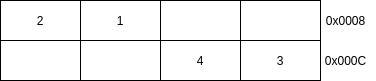
\includegraphics[width=200px]{images/14_Endianness_e_allineamento/accesso_disallineato.png}
    \end{figure}
    per leggere il valore dovrei leggere le due righe e poi ri-assemblare il valore ottenuto per metterlo nel registro.
    
    Gli accessi non allineati sono molto meno efficienti!
\end{itemize}

Altre CPU come AVR invece danno un indirizzo alla riga, 2 byte, non alla singola cella.
Inoltre le occasioni per eseguire accessi non allineati sono molto poche dato che la SRAM ha accessi a byte.

ARM si rifiuta di fare JMP ad indirizzi non multipli di 4.
Intel invece ha gli accessi allineati facoltativi per retrocompatibilità.
Altri processori se si fa un accesso non allineato leggono male senza dare errori.

Ci sono alcune direttive per imporre l' allineamento:
\begin{verbatim}
    .ALIGN(2)
        ; allinea il location_counter a 2
\end{verbatim}
tuttavia spesso conviene evitare di usarle in quanto portano a spreco di memoria utile quando è poca.
Ad esempio nelle strutture del C, che tende ad inserire tutto allineato il più possibile ci sono molti spazi vuoti di \emph{padding}, spesso conviene richiedere al compilatore la soppressione del padding per risparmiare spazio.

